\input{configuration}


\title{Lecture 19 --- Query Optimization}

\author{Jeff Zarnett\\ \small \texttt{jzarnett@uwaterloo.ca}}
\institute{Department of Electrical and Computer Engineering \\
  University of Waterloo}
\date{\today}


\begin{document}

\begin{frame}
  \titlepage

\end{frame}

\begin{frame}
\frametitle{Query Processing}

Imagine you are given an assignment in a course and you are going to do it now. 

\begin{center}
	\includegraphics[width=0.5\textwidth]{images/doitnow.jpg}
\end{center}

You will probably: 

(1) Figure out what exactly the assignment is asking you to do; 

(2) Figure out how you are going to do it; and finally 

(3) Do it! 

\end{frame}

\begin{frame}
\frametitle{Feeling Lost?}

\begin{center}
	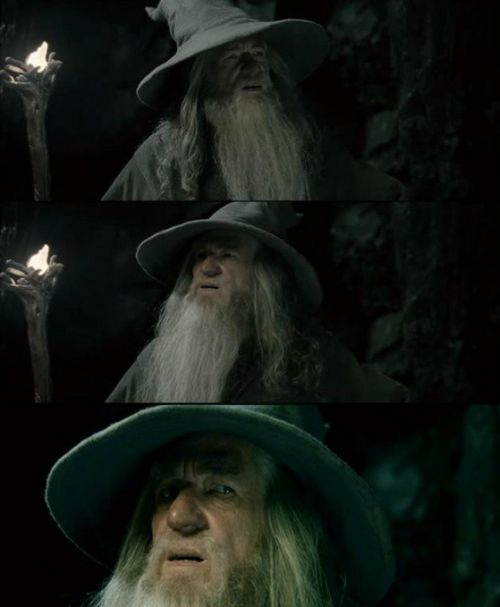
\includegraphics[width=0.4\textwidth]{images/gandalf.png}
\end{center}

We're focusing on step two here.

The database is just a concrete example of the idea.

\end{frame}


\begin{frame}
\frametitle{Query Processing}

The procedure for the database server to carry out the query are the same

\begin{enumerate}
	\item Parsing and translation
	\item Optimization
	\item Evaluation
\end{enumerate}

\end{frame}

\begin{frame}
\frametitle{Adapt, Improvise, and Overcome}

The DB server does not just execute a pre-planned series of steps.

Yes, it's executing the (unchanging) binary code...\\
\quad But the path taken varies based on factors known only at runtime!

\end{frame}

\begin{frame}
\frametitle{Steps Breakdown}
Scan to figure out where the keywords are and what is what.

Check SQL syntax; then the names of attributes and relations.

Make a query graph, which is used to devise the execution strategy. 

Follow the plan.

\end{frame}



\begin{frame}
\frametitle{Do Skip Steps!}

We will not spend time talking about the scanning, parsing, and verification steps of query processing.

\begin{center}
\includegraphics[width=0.4\textwidth]{images/syntaxerror.jpg}
\end{center}

A query with an error is rejected and goes no further through the process. 

\end{frame}

\begin{frame}
\frametitle{Start with SQL}
Usually a query is expressed in SQL and that must then be translated into an equivalent \alert{relational algebra} expression. 

Complex SQL queries are typically turned into \alert{query blocks}, which are translatable into relation algebra expressions. 

A query block has a single select-from-where expression, as well as related group-by and having clauses; nested queries are a separate query block.

\end{frame}

\begin{frame}
\frametitle{Select Your Choice}
A query like \texttt{SELECT salary FROM employee WHERE salary > 100000;} consists of one query block. 

We can select all tuples where salary is more than 100~000 and then perform a projection of the salary field of that result. 

The alternative is to do the projection of salary first and then perform the selection on the cut-down intermediate relation.

\end{frame}


\begin{frame}
\frametitle{Select with Subquery}

\texttt{SELECT name, street, city, province, postalCode FROM address WHERE id IN (SELECT addressID FROM employee WHERE department = 'Development');}. 

Then there are 2 query blocks, 1 for the subquery and 1 for the outer query. 

If there are multiple query blocks, then they do not have to follow the same strategy; they can be optimized separately if desired. 

\end{frame}


\begin{frame}
\frametitle{Make the Plan}


What we need instead is a \alert{query execution plan}.

\begin{center}
	\includegraphics[width=0.5\textwidth]{images/cunningplan.jpg}
\end{center}


To build that up, each step of the plan needs annotations that specify how to evaluate the operation. 
\end{frame}


\begin{frame}
\frametitle{Make the Plan}



This includes information such as what algorithm or what index to use. 

An algebraic operation with the associated annotations about how to get it done is called an \alert{evaluation primitive}. 

The sequence of these primitives forms the plan, that is, how exactly to execute the query.

\end{frame}

\begin{frame}
\frametitle{Time for Plan B}

If there are multiple possible way to carry out the plan, the system will need to make some assessment about which plan is the best. 

It is not expected that users will write optimal queries.

The database server should choose the best approach via \alert{query optimization}. 

Although maybe optimization isn't the right word...

\end{frame}

\begin{frame}
\frametitle{At What Cost?}

If you are asked to drive a car from point A to point B...

\begin{center}
	\includegraphics[width=0.75\textwidth]{images/optimize-map.png}
\end{center}

How does google present the time estimate here?

\end{frame}

\begin{frame}
\frametitle{At What Cost?}

We need to break it down into different sections, such as drive along University Avenue, then get on Highway 85, then merge onto 401... 

By combining all of the segments, you get an estimate of how long that particular route will take. 

If you do this for all viable routes, you can see which route is the best. 

\end{frame}

\begin{frame}
\frametitle{Every Month is Bad Lane Change Month}

If there is a crash on the highway, traffic really sucks and your decision that taking this particular route would be fastest turns out to be wrong. 

\begin{center}
	\includegraphics[width=0.7\textwidth]{images/map-traffic.png}
\end{center}

Short of being able to see into the future, this is more or less inevitable.

\end{frame}

\begin{frame}
\frametitle{Execution Time}

Where does the time go in executing a query? 

The biggest component is most likely loading blocks from disk, considering how slow the disk operations are. 

In reality, CPU time is a nonzero part of query optimization, but we will ignore this for simplicity's sake and use only the disk accesses to assess cost.

\end{frame}

\begin{frame}
\frametitle{Think Disk}

The number of block transfers and the number of disk seeks are the important measures of interest here.
 
To compute the estimate of how long we think it will take to perform an operation, the formula is $b \times t_{T} + S \times t_{s}$. 

For a hard drive, transfer times are on the order of 0.1~ms and seek times are about 4~ms.

\end{frame}

\begin{frame}
\frametitle{Estimation Strategy Caveats}

\begin{center}
	\includegraphics[width=0.7\textwidth]{images/legaleagle.jpg}
\end{center}

Usually we imagine the worst case scenario.

\end{frame}



\begin{frame}
\frametitle{Estimates of Work}

The estimates calculate only the amount of work that we think it will take to complete the operation. 

Unfortunately, there are several factors that will potentially affect the actual wall-clock time it takes to carry out the plan. 

What do you think they are?


\end{frame}



\begin{frame}
\frametitle{Estimates of Work}

\begin{itemize}
	\item How busy the system is
	\item What is in the buffer
	\item Data layout
\end{itemize}


Remember: the lowest cost approach is not necessarily the fastest!

\begin{center}
	\includegraphics[width=0.5\textwidth]{images/greenhillszone.png}
\end{center}

\end{frame}


\begin{frame}
\frametitle{Equivalents: Alternative Routes}

There are many rules to transform a query into an alternative/equivalent.

We aren't going to learn the rules here.

Analogy: in math class you would have learned...\\
\quad $3 \times 10 \times 7$ is the same as $7 \times 10 \times 3$;\\
\quad $14 \times 13$ is the same as $14 \times 10 + 14 \times 3$.


\end{frame}



\begin{frame}
\frametitle{Query Optimization}

Suppose our query involves a selection and a join. 

We want to select the employee number, salary, and address for an employee with an ID of 385. 

Suppose number and salary are in the employee table with 300 entries, and the address information is in another table with 12000 entries. 

\end{frame}

\begin{frame}
\frametitle{Query Optimization}


Bad approach: we will compute the join of employees and addresses, producing 300 results; then select and project on the intermediate result.

If done efficiently, we will do the selection and projection first, meaning the join needs to match exactly one tuple of employees rather than all 300. 

\end{frame}

\begin{frame}
\frametitle{Query Optimization}
The query optimizer should systematically generate equivalent expressions. 

It is likely that the optimizer does not consider every possibility and will take some ``shortcuts'' rather than brute force this. 


\begin{center}
	\includegraphics[width=0.2\textwidth]{images/spock-remember.jpg}
\end{center}

Idea: re-use common subexpressions to reduce the amount of space used by representing the expressions during evaluation.

\end{frame}

\begin{frame}
\frametitle{Evaluation Plan Selection}


\begin{center}
	\includegraphics[width=0.5\textwidth]{images/overthink.jpg}
\end{center}

These operations are not free in terms of CPU usage or time and it is possible to waste more time on analysis than choosing a better algorithm would save. 

\end{frame}


\begin{frame}
\frametitle{Evaluation Plan Selection - Join Focus}

A simplified approach, then, focuses just on what order in which join operations are done and then how those joins are carried out. 

The theory is that the join operations are likely to be the slowest and take the longest, so any optimization here is going to have the most potential benefit.


\begin{center}
	\includegraphics[width=0.7\textwidth]{images/joinus.jpg}
\end{center}

\end{frame}

\begin{frame}
\frametitle{Focus on the Join}

The order of joins in a statement like $r_{1} \bowtie r_{2} \bowtie r_{3}$ is something the optimizer can choose. 

In this case there are 3 relations and there are 12 different join orderings. 

For $n$ relations there are $\dfrac{(2(n-1))!}{(n-1)!}$ possible orderings (some symmetric).


\end{frame}


\begin{frame}
\frametitle{Why Are We Doing This?}

Why joining so many tables? Is this a design issue?

\begin{center}
	\includegraphics[width=0.5\textwidth]{images/zoidberg.jpg}
\end{center}


It cannot examine all (non-symmetric) approaches and choose the optimal one. It would take too long.

\end{frame}


\begin{frame}
\frametitle{Remember Your History}

We can create an algorithm that can ``remember'' subsets of the choices. 

Request  $r_{1} \bowtie r_{2} \bowtie r_{3} \bowtie r_{4} \bowtie r_{5}$? Compute the best order for $(r_{1} \bowtie r_{2} \bowtie r_{3})$. 

Then re-use that repeatedly for any further joins with $r_{4}$ and $r_{5}$. 

This ``saved'' result can be re-used repeatedly.

\end{frame}

\begin{frame}
\frametitle{Make the DB Server Sad}

The resultant approach may not be globally optimal (just locally optimal). 

If $r_{1} \bowtie r_{4}$ produces very few tuples, it may be maximally efficient to do that join computation first.

That will never be tried in an algorithm where $r_{1}$, $r_{2}$, and $r_{3}$ are combined to a subexpression for evaluation. 

\end{frame}

\begin{frame}
\frametitle{It's Not Hard Data}

Remember though, this is as estimating process. 

\begin{center}
	\includegraphics[width=0.7\textwidth]{images/guessing.png}
\end{center}

\end{frame}

\begin{frame}
\frametitle{May You Live In Interesting Times}

The sort order in which tuples are generated is important if the result will be used in another join. 

A sort order is called \alert{interesting} if it is useful in a later operation. 

\end{frame}

\begin{frame}
\frametitle{May You Live In Interesting Times}

Suppose $r_{1}$ and $r_{2}$ are being computed for a join with $r_{3}$.

It is advantageous if the combined result $r_{1} \bowtie r_{2}$ is sorted on attributes that match to $r_{3}$ to make that join more efficient.

If it is sorted by an attribute not in $r_{3}$, an additional sort will be necessary.

\end{frame}

\begin{frame}
\frametitle{Generalizations Are Always Wrong}

The best plan for computing a particular subset of the join query is not necessarily the best plan overall. 

That extra sort may cost more than was saved by doing the join itself faster. 

This increases the complexity, obviously, of deciding what is optimal. 

Fortunately there are, usually anyway, not too many interesting sort orders...

\end{frame}

\begin{frame}
\frametitle{Estimating Statistics}

If we want to know, however, how many employees have a salary between \$40~000 and \$50~000, the only way to be sure is to actually do the query.

\begin{center}
	\includegraphics[width=0.5\textwidth]{images/nuke-from-orbit.jpg}
\end{center}

And we don't want to do the query when estimating the cost...

\end{frame}


\begin{frame}
\frametitle{Guess we better... guess?}

If we cannot measure, then, well, we need to guess.

No need to be perfect: all we need is to be better than not optimizing!

\end{frame}

\begin{frame}
\frametitle{Cost Centres}

Areas where costs for performing a query accumulates:

\begin{enumerate}
	\item \textbf{Disk I/O}
	\item \textbf{Disk Additional Storage}
	\item \textbf{Computation}
	\item \textbf{Memory}
	\item \textbf{Communication}
\end{enumerate}

Assumption: disk is the largest one.

\end{frame}


\begin{frame}
\frametitle{Metadata}

Some items that might be in the metadata:

\begin{itemize}
	\item $n_{r}$: the number of tuples in a relation $r$ 
	\item $b_{r}$: The number of blocks containing a relation $r$ 
	\item $l_{r}$: the size in bytes of relation $r$
	\item $f_{r}$: the number of tuples of $r$ that fit into one block
	\item $V(A, r)$: the number of distinct values in $r$ of attribute $A$
	\item $h_{r, i}$: the height of an index $i$ defined on relation $r$
\end{itemize}

There can also be metadata about index information as well... which might make it metametadata?

\end{frame}



\begin{frame}
\frametitle{Maintaining Metadata}

The more often it is updated, the more effort is spent updating it. 

If every insertion or update or deletion resulted in an update, that may mean a nontrivial amount of time is spent updating this data. 

If we only do periodic updates, it likely means that the statistic data will be outdated when we go to retrieve it for use in a query optimization context. 

Perhaps some amount of balance is necessary...


\end{frame}

\begin{frame}
\frametitle{Histogram Data}

A database may also be interested in keeping some statistical information in a histogram. 

The values are divided into ranges and we have some idea of how many tuples are in those ranges. 

\begin{center}
\includegraphics[width=0.4\textwidth]{images/histogram}
\end{center}

\end{frame}

\begin{frame}
\frametitle{Estimating Metadata}

The above numbers are exact values which we can know and, hopefully, trust. 

Although they could be slightly out of date depending on when exactly metadata updates are performed. 

The more exact values we have, the better our guesses. But things start to get interesting when we ask something that does not have a category.


\end{frame}


\begin{frame}
\frametitle{Join Elimination}

Slight digression on \alert{Join Elimination}.

Attempt to eliminate the join altogether if it can be skipped. 

The optimizer can only do this if there is certainty that the outcome will not be affected by not doing the join. 


\end{frame}

\begin{frame}
\frametitle{Join Elimination}

You may ask, of course, why should the optimizer do this work at all? 

Why not simply count on the developers who wrote the SQL in the first place to refactor/change it so that it is no longer so inefficient? 

Grind leetcode (please no) and git gud (seriously wtf).


\begin{center}
	\includegraphics[width=0.2\textwidth]{images/wantitall.jpg}
\end{center}
\end{frame}

\begin{frame}
\frametitle{Join Elimination}


Regardless, SQL is a language in which you specify the result that you want, not specifically how to get it. 


Compilers don't admonish the user for writing code that it has to transform into a faster equivalent, they just do that transparently.


\end{frame}

\begin{frame}
\frametitle{Join Elimination Example}

Query: \texttt{SELECT c.* FROM customer AS c JOIN address AS a ON c.address\_id = a.address\_id;} 


Inner join; as presented, cannot eliminate.

We need to make sure that the customer data has a matching row.


\end{frame}

\begin{frame}
\frametitle{Eliminate the Join}

Suppose that we have a foreign key defined from customer's \texttt{address\_id} to the address \texttt{id} field. 

If nulls are not permitted, then we know for sure that every customer has exactly one record in the address table.

Therefore the join condition is not useful and may be eliminated. 

New query: \texttt{select * from customer;} faster (select without conditions).


\end{frame}

\begin{frame}
\frametitle{More Elimination}

The foreign key and not null constraints on the address ID field of the customer enable elimination.

An outer join constraint can be removed as well.

Imagine the query said this: \texttt{SELECT c.* FROM customer AS c LEFT OUTER JOIN address AS a ON c.address\_id = a.address\_id;}. 

All tuples are fetched from customer whether or not there is an address. 

\end{frame}

\begin{frame}
\frametitle{Or Don't...?}

If, however, both constraints are removed and we cannot be sure that there is at most one address corresponding to a customer.

Then we have to do the join.


\end{frame}

\begin{frame}
\frametitle{Harder to Read}
Obviously, the more complex the query, the harder it is to determine whether or not a particular join may be eliminated. 

The same queries written on a database in which the constraints have not been added would not be eligible for the join elimination optimization. 

This reveals a second purpose why constraints are valuable in the database.

\end{frame}

\begin{frame}
\frametitle{Join Elimination Analogy}
Task: find all copies of the book ``Harry Potter and the pthread House Elves''. 


\begin{center}
	\includegraphics[width=0.5\textwidth]{images/archives.jpg}
\end{center}

Rule: this library will keep only one copy of that book ever. 

As soon as you have found the single copy of that book, you can stop looking.

\end{frame}

\begin{frame}
\frametitle{Shortcuts}

Now we will talk about some heuristic rules (guidelines, really) that we have definitely mentioned earlier.


\end{frame}

\begin{frame}
\frametitle{Perform selection early}

No surprises here: the sooner we do a selection, the fewer tuples are going to result and the fewer tuples are input to any subsequent operations. 


There are exceptions, however: if we throw away too much, it forces us to do a full table scan to complete a join. 


\end{frame}

\begin{frame}
\frametitle{Perform projection early}

Analogous to the idea of doing selection early, performing projection early is good because it tosses away information we do not need.

Just like selection, however, it is possible the projection throws away an attribute that will be useful.


\end{frame}

\begin{frame}
\frametitle{Set Limits}

Another strategy for making sure we choose something appropriate within a reasonable amount of time is to set a time limit. 

Optimization has a certain cost and once this cost is exceeded, the process of trying to find something better stops. 

But how much time to we decide to allocate? 


\end{frame}

\begin{frame}
\frametitle{Plan Caching}

In any busy system, common queries may be repeated over and over again with slightly different parameters. 

A student wishes to query what courses they are enrolled in. 

If one student does this query with a particular value for student ID number, we can re-use that same evaluation plan in the future.

\end{frame}


\begin{frame}
\frametitle{Estimating Statistics}

In the previous example I used exact numbers, 300... 1... 12000... etc.,

But for the database server to get those it can either look them up, or it can guess about them. 

As mentioned earlier, sometimes certain numbers, like the number of tuples in a relation, are easily available by looking at metadata. 

\end{frame}


\begin{frame}
\frametitle{Applicability}

If we're not implementing a database is this still useful?

Yes -- the database is just an example!

Real lesson: how to programmatically generate, evaluate, and choose amongst alternatives.

\end{frame}


\end{document}

